\documentclass[10pt]{article}

% Lines beginning with the percent sign are comments
% This file has been commented to help you understand more about LaTeX

% DO NOT EDIT THE LINES BETWEEN THE TWO LONG HORIZONTAL LINES

%---------------------------------------------------------------------------------------------------------

% Packages add extra functionality.
\usepackage{times,graphicx,epstopdf,fancyhdr,amsfonts,amsthm,amsmath,algorithm,algorithmic,xspace,hyperref}
\usepackage[left=1in,top=1in,right=1in,bottom=1in]{geometry}
\usepackage{sect sty}	%For centering section headings
\usepackage{enumerate}	%Allows more labeling options for enumerate environments 
\usepackage{epsfig}
\usepackage[space]{grffile}
\usepackage{booktabs}
\usepackage{forest}
\usepackage{enumitem}   
\usepackage{fancyvrb}
\usepackage{todonotes}
\usepackage{setspace}


% This will set LaTeX to look for figures in the same directory as the .tex file
\graphicspath{.} % The dot means current directory.

\pagestyle{fancy}

\lhead{Final Project}
\rhead{\today}
\lfoot{CSCI 334: Principles of Programming Languages}
\cfoot{\thepage}
\rfoot{Spring 2024}

% Some commands for changing header and footer format
\renewcommand{\headrulewidth}{0.4pt}
\renewcommand{\headwidth}{\textwidth}
\renewcommand{\footrulewidth}{0.4pt}

% These let you use common environments
\newtheorem{claim}{Claim}
\newtheorem{definition}{Definition}
\newtheorem{theorem}{Theorem}
\newtheorem{lemma}{Lemma}
\newtheorem{observation}{Observation}
\newtheorem{question}{Question}

\setlength{\parindent}{0cm}

%---------------------------------------------------------------------------------------------------------

% DON'T CHANGE ANYTHING ABOVE HERE

% Edit below as instructed

\title{Twined Language Specification} % Replace SnappyLanguageName with your project's name

\author{Lucas Weissman \and Zach Sturdevant} % Replace these with real partner names.

\begin{document}
  
\maketitle

\subsection*{Introduction}

2+ paragraphs. What problem does your language solve? What makes you think that this problem
 should have its own programming language?

"Twined" represents a transformative approach in how we manage and interact
 with textual information. By converting unstructured text data from diverse 
 note-taking formats into structured, navigable knowledge graphs, "Twined" 
 provides a unique visual perspective that enhances comprehension and analysis.

 Twinned should be a programing language becausee of how much time it takes to
 learn and impliment programs required to achieve a similar output.
 By making a programing language we can handle the implimentation details
 and increase accessibility to tools that promote learning and understanding. 
 \singlespacing


 Rules:
 Graph Rule: {x, y}, {x, z} → {x, z}, {x, w}, {y, w}, {z, w}
 \singlespacing
 Hypergraph Rule: {x, y, z} → {x, u, v}, {z, v, w}, {y, w, u}
 \singlespacing


 graph: {Sunlight,Plant Growth},{Water,Plant Growth},{Soil Nutrients,Plant Growth}
 \singlespacing
 hypergraph: {Sunlight,Water,Soil Nutrients,Plant Growth},{Temperature,Humidity,Water,Plant Growth}
 \singlespacing

Brainstorming Section:

“Twined” intertwines user’s information by managing and interacting with textual 
information. It converts unstructured text data from various note-taking formats 
into structured, navigable knowledge graphs. This will allow users to quickly 
visualize connections and gain insights that might be missed in traditional 
textual data formats. 

\singlespacing
A hypergraph is defined as a collection of nodes and hyperedges, where each 
hyperedge has the capability to connect three or more nodes, unlike traditional
graphs where edges connect only two nodes. In terms of mathematical 
representation, edges in standard graphs are noted as pairs of numbers within 
curly brackets, such as {1, 2}. Conversely, in hypergraphs, hyperedges 
that connect multiple nodes are denoted by three or more numbers within 
curly brackets, for example, {1, 2, 3}. Visually, in graphs, edges are depicted
as connections between white dots (nodes) using white arrows (edges). 
Hypergraphs extend this visualization by linking three or more white dots 
(nodes) with multiple arrows and a transparent white web, highlighting the
complex relationships between nodes.

\singlespacing
PS. We might adjust the intro to fit within the context of our current 
deliverables, or we could state the end goal briefily and current stage 
we are in with the test cases we have built. - Lucas

\newpage
\subsection*{Design Principles}

1+ paragraphs. Languages can solve problems in many ways. What are the aesthetic or technical 
ideas that guide its design?

\singlespacing
The goal of this language is to produce useful output with minumal input from the user in an easy to understand
way. In the current form the user has to design and build the graph themselves, but as continue we plan to add
features that will allow the user to upload a text and say in english what they hope to get out of it and the
language will handle the rest. Aesthetic we are attempting to have a simple start that move into a powerful 
GUI to allow anyone to use the language. 

From a technical stand point we want to utilize generative AI to imporve the ability of people to access
knowledge in a way that is efficient and allows for multiple kinds of inputs and customization of the
outputs. Basically use technoligy to make peoples lives better and make knowledge more readily accessable
to all.
\singlespacing

Brainstorming Section:


\newpage
\subsection*{Examples}
\begin{enumerate}
  \item 
    \begin{enumerate}
      \item Program 1 input
        \begin{verbatim}
          {Nancy, (Fred, Sally, Sarah,)}
          {Fred, (Nancy, Sally, Sarah,)}
          {Sally, (Jeff, Jonny, Timmy,)}
          {Jeff, (Sally, Jonny, Timmy,)}
        \end{verbatim}
      \item Program 1 output
        \begin{figure}[!hb]
          \centering
          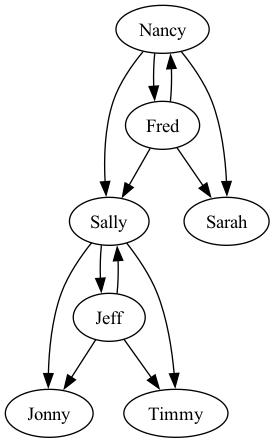
\includegraphics[width=0.3\linewidth]{images/family_tree.png} 
          \caption{Family Relationship}
          \label{figure 1:}
        \end{figure}
      \item
        This graph represents the relationships between family individuals. Each node represents 
        a person, and each edge represents a direct relationship between two individuals. For example,
        "Nancy" has relationships with "Sally," "Fred," and "Sarah," as depicted by the edges 
        connecting their respective nodes.
    \end{enumerate}
  \item
    \begin{enumerate}
      \item Program 2 input
        \begin{verbatim}
          {Sunlight, (PlantGrowth,)}
          {Water, (PlantGrowth,)}
          {SoilNutrients, (PlantGrowth,)}
        \end{verbatim}
      \item Program 2 output
        \begin{figure}[!hb]
          \centering
          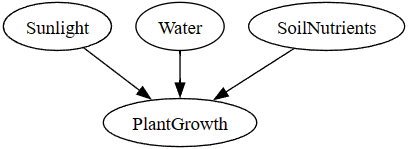
\includegraphics[width=0.4\linewidth]{images/plant_test_0.1.png} 
          \caption{Plant Growth Relationship}
          \label{figure 2:}
        \end{figure}
      \item
        The graph represents factors affecting plant growth. Each node represents
        a factor such as "Sunlight," "Water," and "Soil Nutrients," and each edge 
        represents the influence of these factors on "Plant Growth," as depicted 
        by the edges connecting their respective nodes.
    \end{enumerate}
  \item
    \begin{enumerate}
      \item Program 3 input
        \begin{verbatim}
          {European Fascism, (Germany, Italy, Spain,)}
          {Germany, (Adolf Hitler,)}
          {Italy, (Benito Mussolini,)}
          {Spain,(Francisco Franco,)}
        \end{verbatim}
      \item Program 3 output
        \begin{figure}[!hb]
          \centering
          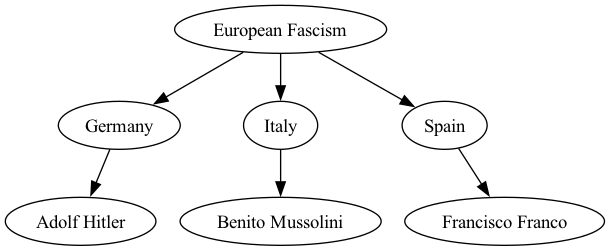
\includegraphics[width=0.5\linewidth]{images/Fascism.png} 
          \caption{Famious Eureopean Fascists}
          \label{figure 3:}
        \end{figure}
      \item
        This graph shows connections between European Fascism and leaders 
        of different Fascist countries. Each node represents a topic and 
        how those topics are connected in a top down manner.
    \end{enumerate}
\end{enumerate}


\singlespacing

Brainstorming Section
\singlespacing

I have added above an example of image insertion from one of our test cases, we could replace 
it with a few more/new ones. - Lucas

\newpage
\subsection*{Language Concepts}
(What are the core concepts a user needs to understand in order to write programs? 
Think in terms of both “primitives” and “combining forms.” What are the key ideas and 
how are they combined?)

Currently the user needs to understand how graph nodes connect. However when comepleted the
user shouldn't need an understanding of primatives, just input the information they want to explore
and utilize the GUI to explore the information.

The language concepts behind "Twined" incorporate elements from graph theory 
and data visualization to support the creation of knowledge graphs and 
hypergraphs. These concepts are integral in defining how textual data is parsed, 
how entities within the text are identified as nodes, and how relationships (edges)
are established based on the context and content of the data. This allows "Twined"
to dynamically interpret and display information in a way that highlights
both hierarchical and associative relationships.



\singlespacing
\todo[inline]{Delete this TODO and replace with 1+ paragraphs.}
\singlespacing

Brainstorming Section

Terms to be used/contextualized:
Graph Theory
Data Visualization
Knowledge Graphs
Hypergraphs
Parsing
Nodes
Edges
Hierarchical Relationships
Associative relationships

\newpage
\subsection*{Formal Syntax}
\singlespacing

\begin{tabular}{lll}
    $<\textbf{expression}>$ & ::= & $<\textbf{Node}>$  \\
                            & $|$  & $<\textbf{edgeList}>$ \\
                            & $|$  & $<\textbf{nodeName}>$ \\
                            & $|$  & $<\textbf{listOfNodes}>$ \\
                            
    $<\textbf{Node}>$   & ::= & \{ $<\textbf{String}>$, $<\textbf{nodeName}>$ \} \\
    $<\textbf{nodeName}>$& ::= &  $<\textbf{String}>$ \\
    $<\textbf{edgeList}>$& ::= & ($<\textbf{nodeName}>$ +) \\
    $<\textbf{listOfNodes}>$& ::= & $<\textbf{Node}>$ + \\
    
    \end{tabular}

\singlespacing   
\todo[inline]{Delete this TODO and replace with BNF.}
\singlespacing

\begin{center}
    \begin{forest}
      [{$<\textbf{expression}>$} 
        [{$<\textbf{abstraction}>$}
          [{$\lambda<\textbf{variable}>$}
            [{$x$}]
          ]
          [{$<\textbf{expression}>$} 
            [{$<\textbf{application}>$}
              [{$<\textbf{expression}>$}
                [{$<\textbf{variable}>$}
                  [{x}]
                ]
              ]
              [{$<\textbf{expression}>$}
                [{$<\textbf{variable}>$}
                  [{y}]
                ]
              ]
            ]
          ]
        ]
      ]
    \end{forest}
  \end{center}

Brainstorming Section

\newpage
\subsection*{Semantics}
    \begin{enumerate}
      \item Primitive values:
        \begin{enumerate}
          \item NodeName: A series of characters digits or spaces that represent the name of a node. stored in
          a string.
          \item EdgeList: A series of NodeNames, or 0 stored in the form (NodeName, NodeName,) 
          that contains the NodeNames of nodes connected to the node, stored in a list.
        \end{enumerate}
      \item Combining forms:
        \begin{enumerate}
          \item Node: A tuple of the form {NodeName, (EdgeList)} that represents a full node, which is
          the name of the node and its EdgeList. In the future the node name will be used to access
          a dictionary that contains the information associted with that node
          \item NodeList: A series of nodes in the form Node Node separated by whitespace including newlines
          these are used to represent all nodes in a graph
        \end{enumerate}
      \item Evalutation:
          \begin{enumerate}
            \item The programs in our language read inputs given in a txt file, it parses the text file and
            separating the series of nodes and their edges.
            \item When the program is evaluated it produces a graph using the nodes and their edgelist on the
            screen
          \end{enumerate}
            
          
    \end{enumerate}

\singlespacing

\singlespacing

Brainstorming Section


% DO NOT DELETE ANYTHING BELOW THIS LINE
\end{document}
